\itemhead{4.2 例题 · 例题3（教材p.110）}{XJ-B1-C04-EX-P110-Y0319}
\label{XJ-B1-C04-EX-P110-Y0319}
{\footnotesize 湘教版教材p.110 / PDF第117页 / 4.2 例题 / 例题3}
\field{原题}{作出指数函数 $y=3^x$ 和 $y=10^x$ 的图象。}
\field{参考答案}{分别标点：$3^x$ 经过 $(-1,1/3),(0,1),(1,3)$；$10^x$ 经过 $(-1,1/10),(0,1),(1,10)$，用递增平滑曲线连接，向左逼近 $x$ 轴。$x>0$ 时 $10^x>3^x$；$x<0$ 时反向。}
\begin{center}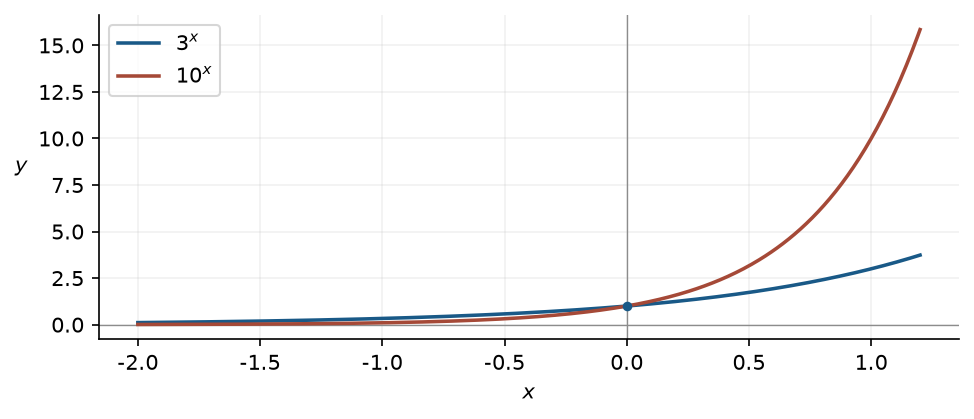
\includegraphics[width=.84\linewidth,height=.38\textheight,keepaspectratio]{figures/C04-EX110-3.png}\end{center}
{\small \field{关联知识}{E01 指数函数的概念、图象与性质（教材帮p.150、151 / PDF159、160）；F04 函数三种表示法、图象与读数（教材帮p.85、86、93、94 / PDF94、95、102、103）}
\field{方法与易错点}{先查底数条件，利用已知点定底数，再据单调性及图象求值或范围。 易错：只要求底数非负；漏排1；将 $a^x+b$ 当标准指数函数且仍用原值域。}
\field{答案依据}{例题原解位置：湘教版教材p.110及题库原图；独立编写可编辑参考解答。答案册此部分主要收练习、习题，不伪造例题答案册位置。}}
